\documentclass[11pt]{article}
\usepackage{multirow}
\usepackage{hyperref}
\usepackage[margin=0.75in, top=1in]{geometry} 
\usepackage{titling} 
\usepackage{fancyhdr}
\usepackage{cancel}
\usepackage{amsmath}
\usepackage{graphicx}
\usepackage{ragged2e}
\usepackage{calc}
\usepackage{here}
\usepackage{siunitx}
\usepackage{float}





\setlength{\droptitle}{-3cm} 
\pagestyle{fancy}
\fancyhf{} 
\lhead{EN.566: Introduction to Computational Materials Modeling 2023 - HW4}
\rhead{Amitabh Roy}

\begin{document}

\section{Problem Description}
The objective of the HW4 is to solve the problem of random numbers, random walks, 1D diffusion and mixing of the gasses. The report will focus on the random numbers and various implementation of those. Detailed explanation for each section can be found in the later section of the report.

\section{Solution to Random Numbers}
Pseudo-Code:
\begin{enumerate}
    \item \textit{Generate uniform random numbers between 0 to 1 using random or numpy modules 1000 random number and 1000000 random number}
    \item \textit{To better visualize the distribution use histogram as we can change the interval size or 'bin' size}
    \item \textit{Convert uniformly distributed random numbers into gaussian distributed ones using the Box-Muller transformation.}
    \item \textit{for box-muller, split the data into 2 equal parts 'u1' and 'u2',  Box-Muller formula to transform u1 and u2 into two sets of normally distributed random numbers, z1 and z2 and then finally combine the z1 and z2}
    \item \textit{Repeat step 2}
    
\end{enumerate}
\subsection{Generation of random numbers with distribution increasing resolution}

\begin{figure}[H]
    \centering
    \begin{minipage}{0.48\textwidth}
        \centering
        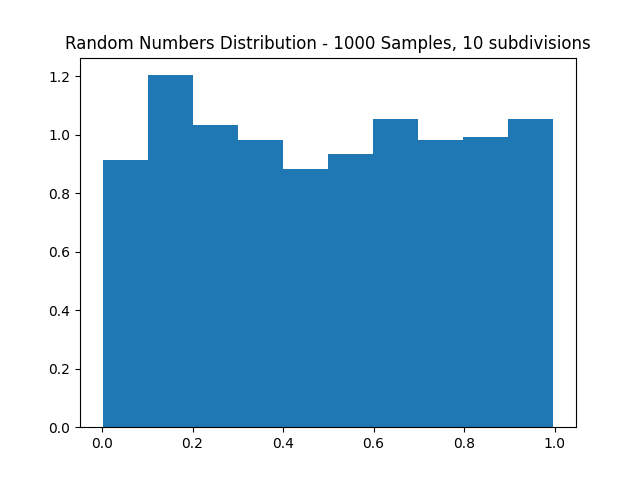
\includegraphics[width=\textwidth]{Random Numbers Distribution - 1000 Samples, 10 subdivisions.png}
        \caption{Random Numbers Distribution - 1000 Samples, 10 subdivisions}
        \label{fig:1}
    \end{minipage}\hfill
    \begin{minipage}{0.48\textwidth}
        \centering
        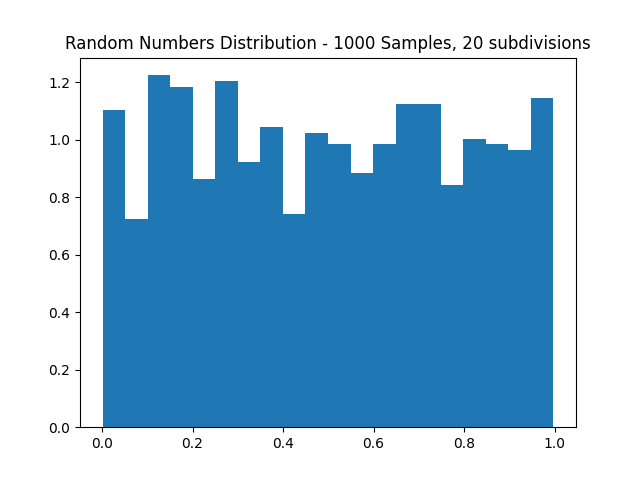
\includegraphics[width=\textwidth]{Random Numbers Distribution - 1000 Samples, 20 subdivisions.png}
        \caption{Random Numbers Distribution - 1000 Samples, 20 subdivisions}
        \label{fig:2}
    \end{minipage}
\end{figure}

\begin{figure}[H]
    \centering
    \begin{minipage}{0.48\textwidth}
        \centering
        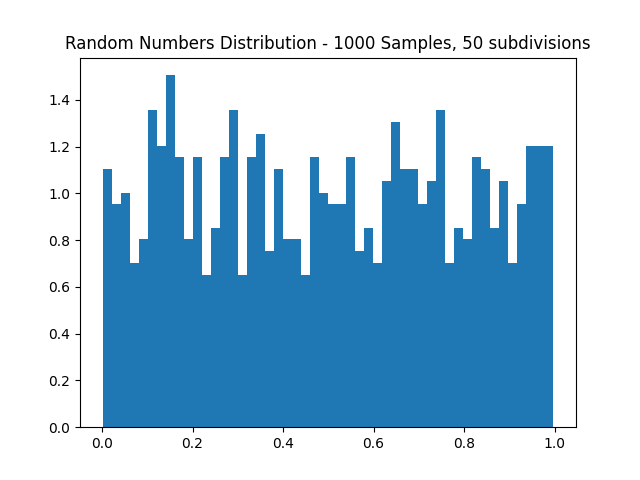
\includegraphics[width=\textwidth]{Random Numbers Distribution - 1000 Samples, 50 subdivisions.png}
        \caption{Random Numbers Distribution - 1000 Samples, 50 subdivision}
        \label{fig:3}
    \end{minipage}\hfill
    \begin{minipage}{0.48\textwidth}
        \centering
        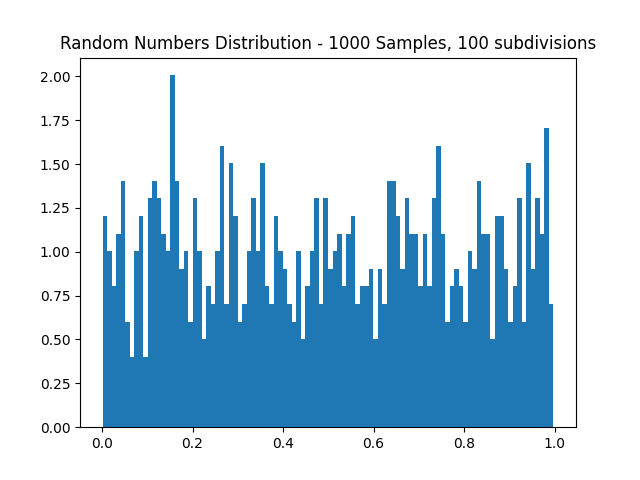
\includegraphics[width=\textwidth]{Random Numbers Distribution - 1000 Samples, 100 subdivisions.png}
        \caption{Random Numbers Distribution - 1000 Samples, 100 subdivisions}
        \label{fig:4}
    \end{minipage}
\end{figure}

\begin{figure}[H]
    \centering
    \begin{minipage}{0.48\textwidth}
        \centering
        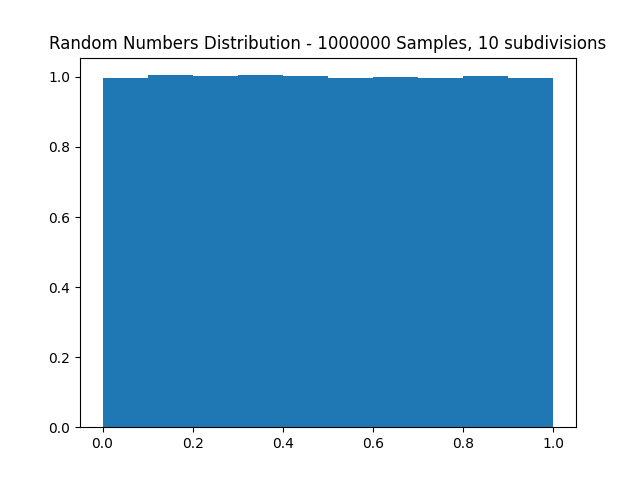
\includegraphics[width=\textwidth]{Random Numbers Distribution - 1000000 Samples, 10 subdivisions.png}
        \caption{Random Numbers Distribution - 1000000 Samples, 10 subdivisions}
        \label{fig:5}
    \end{minipage}\hfill
    \begin{minipage}{0.48\textwidth}
        \centering
        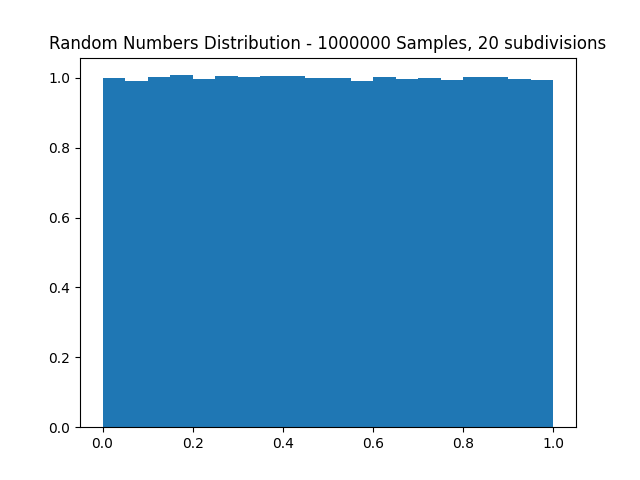
\includegraphics[width=\textwidth]{Random Numbers Distribution - 1000000 Samples, 20 subdivisions.png}
        \caption{Random Numbers Distribution - 1000000 Samples, 20 subdivisions}
        \label{fig:6}
    \end{minipage}
\end{figure}

\begin{figure}[H]
    \centering
    \begin{minipage}{0.48\textwidth}
        \centering
        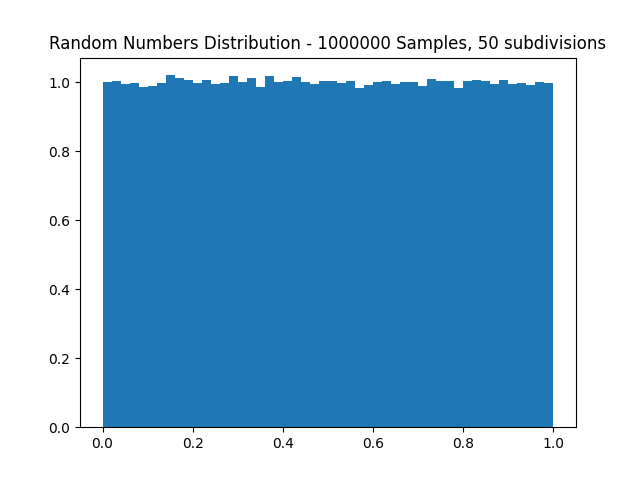
\includegraphics[width=\textwidth]{Random Numbers Distribution - 1000000 Samples, 50 subdivisions.png}
        \caption{Random Numbers Distribution - 1000000 Samples, 50 subdivisions}
        \label{fig:7}
    \end{minipage}\hfill
    \begin{minipage}{0.48\textwidth}
        \centering
        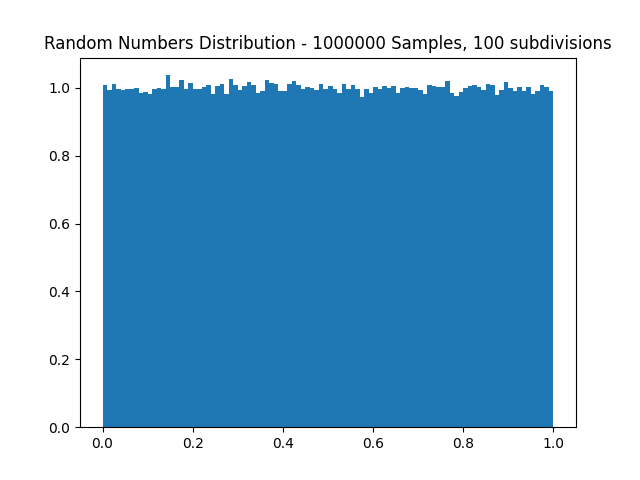
\includegraphics[width=\textwidth]{Random Numbers Distribution - 1000000 Samples, 100 subdivisions.png}
        \caption{Random Numbers Distribution - 1000000 Samples, 100 subdivisions}
        \label{fig:8}
    \end{minipage}
\end{figure}

\subsection{Generation the Gaussian distributed random numbers}
\begin{figure}[H]
    \centering
    \begin{minipage}{0.48\textwidth}
        \centering
        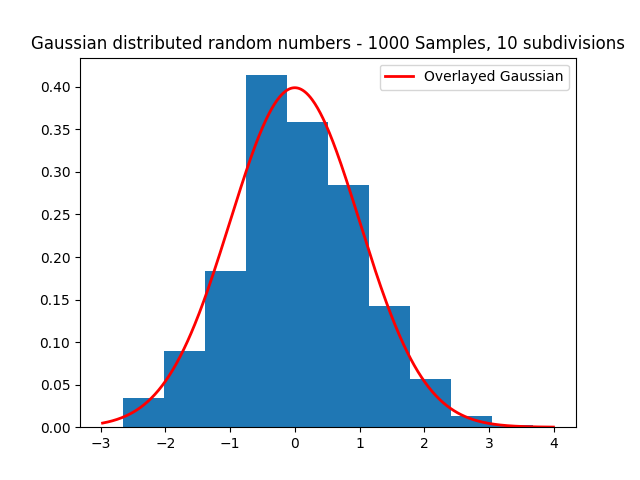
\includegraphics[width=\textwidth]{Gaussian distributed random numbers - 1000 Samples, 10 subdivisions.png}
        \caption{Gaussian distributed random numbers - 1000 Samples, 10 subdivisions}
        \label{fig:9}
    \end{minipage}\hfill
    \begin{minipage}{0.48\textwidth}
        \centering
        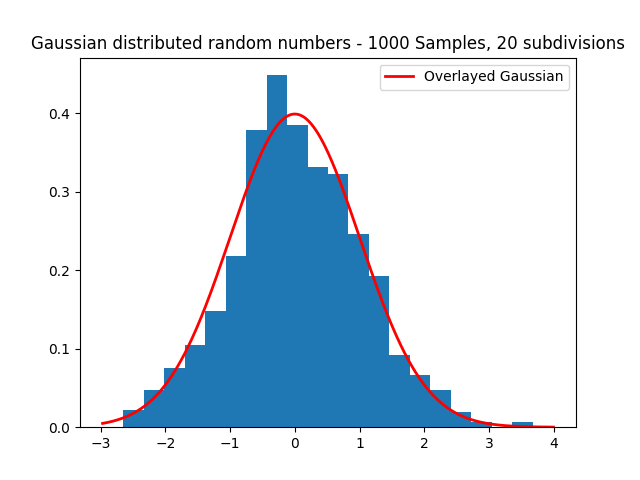
\includegraphics[width=\textwidth]{Gaussian distributed random numbers - 1000 Samples, 20 subdivisions.png}
        \caption{Gaussian distributed random numbers - 1000 Samples, 20 subdivision}
        \label{fig:10}
    \end{minipage}
\end{figure}

\begin{figure}[H]
    \centering
    \begin{minipage}{0.48\textwidth}
        \centering
        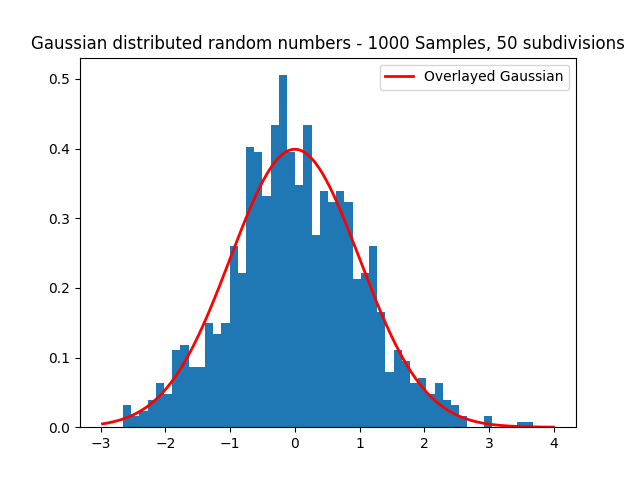
\includegraphics[width=\textwidth]{Gaussian distributed random numbers - 1000 Samples, 50 subdivisions.png}
        \caption{Gaussian distributed random numbers - 1000 Samples, 50 subdivisions}
        \label{fig:11}
    \end{minipage}\hfill
    \begin{minipage}{0.48\textwidth}
        \centering
        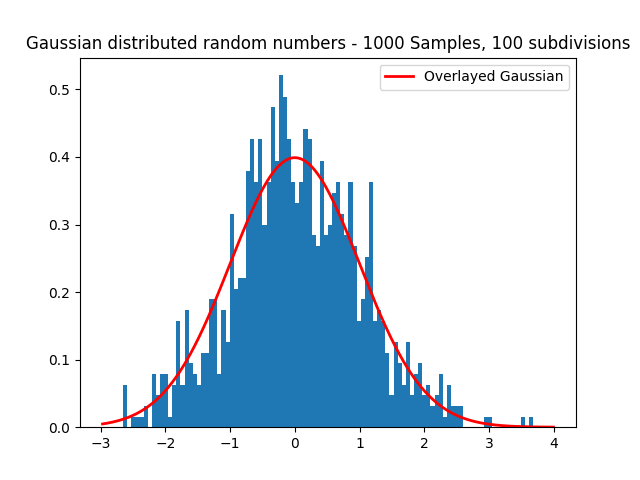
\includegraphics[width=\textwidth]{Gaussian distributed random numbers - 1000 Samples, 100 subdivisions.png}
        \caption{Gaussian distributed random numbers - 1000 Samples, 100 subdivision}
        \label{fig:12}
    \end{minipage}
\end{figure}

\begin{figure}[H]
    \centering
    \begin{minipage}{0.48\textwidth}
        \centering
        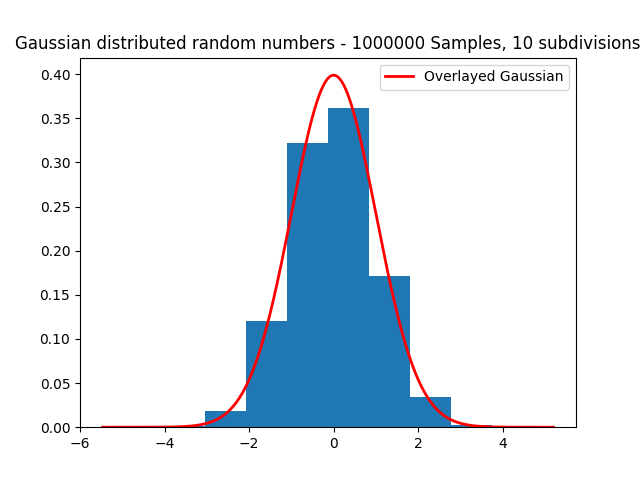
\includegraphics[width=\textwidth]{Gaussian distributed random numbers - 1000000 Samples, 10 subdivisions.png}
        \caption{Gaussian distributed random numbers - 1000000 Samples, 10 subdivisions}
        \label{fig:13}
    \end{minipage}\hfill
    \begin{minipage}{0.48\textwidth}
        \centering
        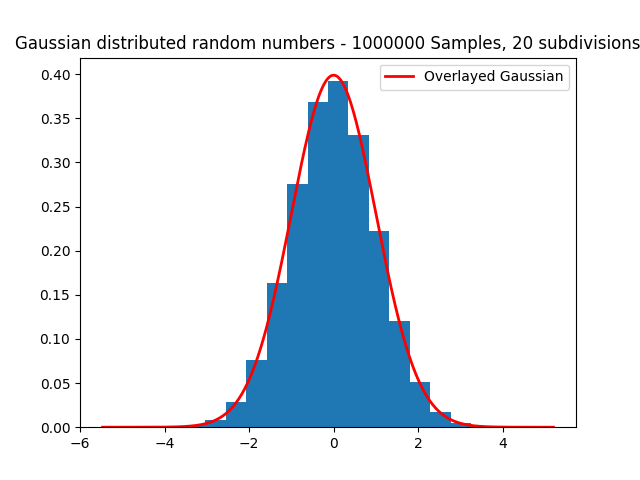
\includegraphics[width=\textwidth]{Gaussian distributed random numbers - 1000000 Samples, 20 subdivisions.png}
        \caption{Gaussian distributed random numbers - 1000000 Samples, 20 subdivisions}
        \label{fig:14}
    \end{minipage}
\end{figure}

\begin{figure}[H]
    \centering
    \begin{minipage}{0.48\textwidth}
        \centering
        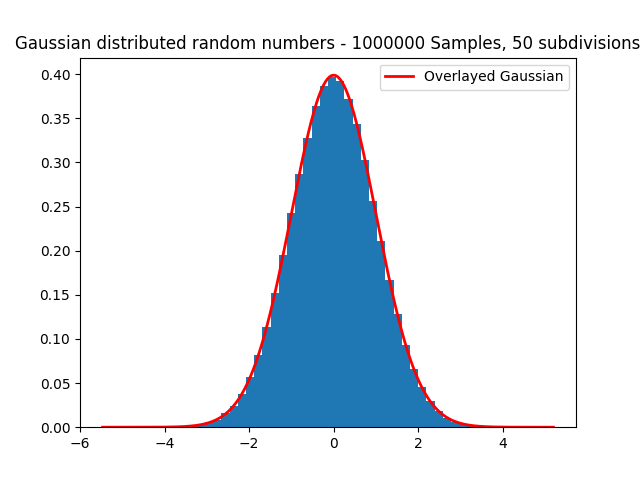
\includegraphics[width=\textwidth]{Gaussian distributed random numbers - 1000000 Samples, 50 subdivisions.png}
        \caption{Gaussian distributed random numbers - 1000000 Samples, 50 subdivisions}
        \label{fig:15}
    \end{minipage}\hfill
    \begin{minipage}{0.48\textwidth}
        \centering
        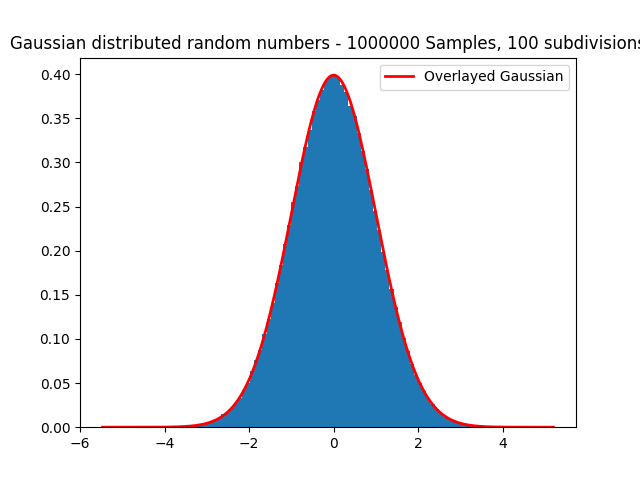
\includegraphics[width=\textwidth]{Gaussian distributed random numbers - 1000000 Samples, 100 subdivisions.png}
        \caption{Gaussian distributed random numbers - 1000000 Samples, 100 subdivisions}
        \label{fig:16}
    \end{minipage}
\end{figure}

\section{2D Random Walk} 
Pseudo-Code:
\begin{enumerate}
    \item \textit{Give equal probability to move up-down-left-right in a 2D, start teh walk from (0,0)}
    \item \textit{For steps less than 3 do only one trials for find the probability of moving and then move}
    \item \textit{Use the end coordinate of the previous step as an starting point for the next step}
    \item \textit{For steps more than 3, take average of 10000 such probability }
    \item \textit{From each walk we will get set of average values for x and y coordinates}
    \item \textit{Plot \( x \) vs steps and \( x^2 \) vs steps.}
    \item \textit{For the mean square distance from the starting point, calculate the value of \( x^2 + y^2 \).}    
\end{enumerate}
\subsection{Average of $<x_n>$ and $<x_n>^2$ up to $n = 100$}
\begin{figure}[H]
    \centering
    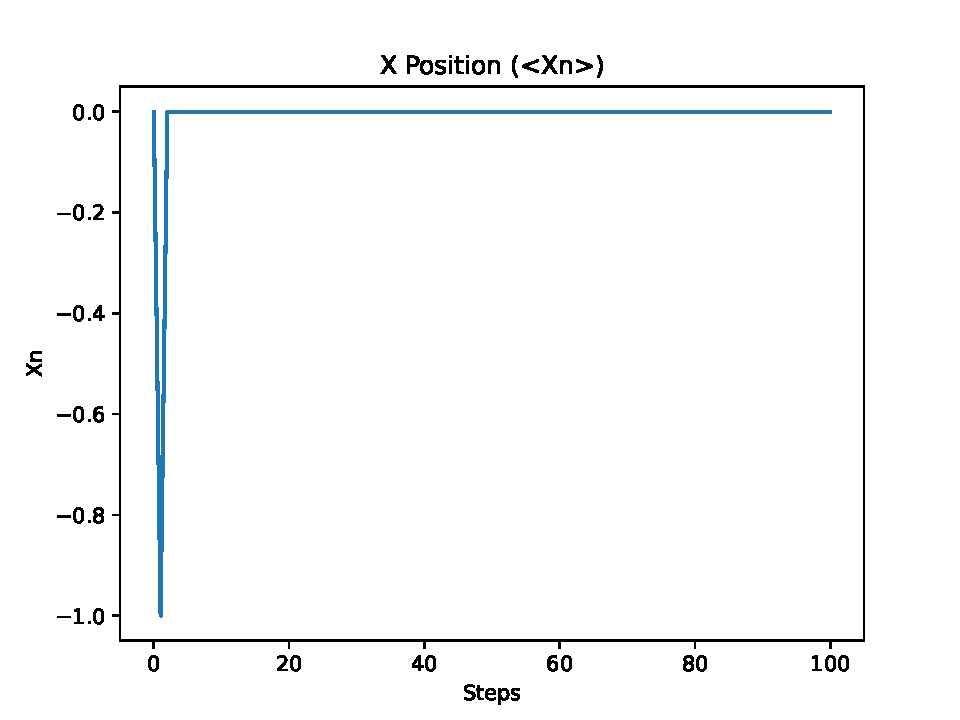
\includegraphics[width=0.48\textwidth, keepaspectratio]{(<Xn>).pdf}
    \caption{Average of \( x_n \)}
    \label{fig:17}
\end{figure}

\begin{figure}[H]
    \centering
    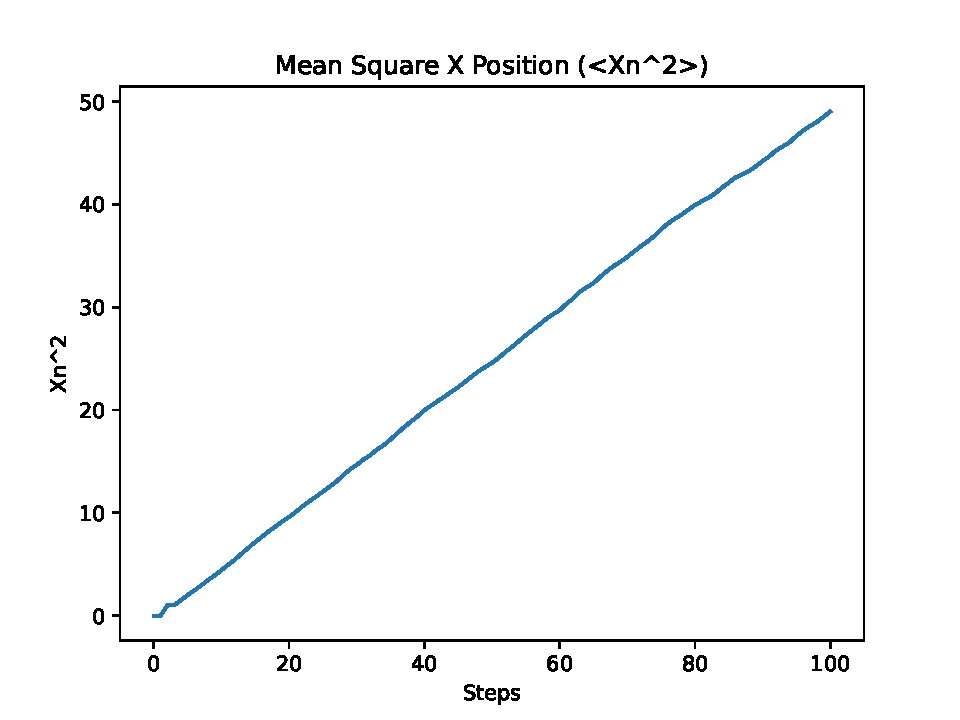
\includegraphics[width=0.48\textwidth, keepaspectratio]{(<Xn>)^2.pdf}
    \caption{Square of the Average of \( x_n \)}
    \label{fig:18}
\end{figure}


\subsection{Mean square distance from the starting point  $<r^2>$ up to $n = 100$}
\begin{figure}[H]
    \centering
    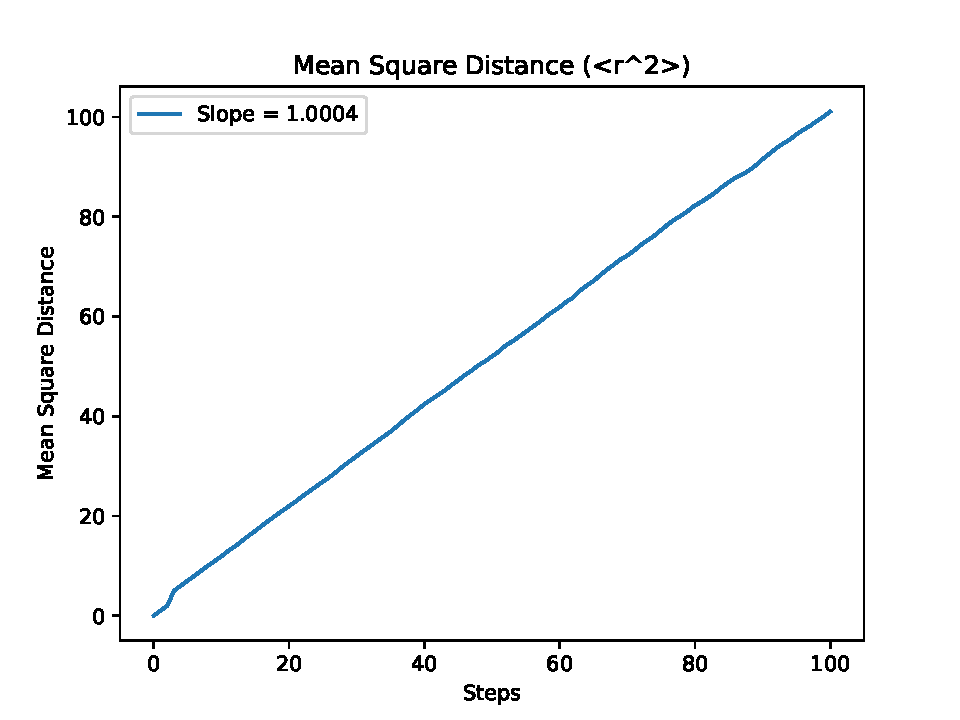
\includegraphics[width=0.48\textwidth, keepaspectratio]{(<r^2>).pdf}
    \caption{Mean square distance from the starting point  $<r^2>$}
    \label{fig:19}
\end{figure}
As shown in Figure~\ref{fig:19}, the slope of the mean squared distance is approximately 1. And as we know: 
\begin{equation}
    r^2 = 4Dt
\end{equation}
In this equation:
\begin{itemize}
    \item \( r \) represents the root mean square displacement
    \item \( D \) is the diffusion constant
\end{itemize}
We can find the value of diffusion constant by dividing the slope with 4, hence the value for diffusion constant = 0.5 (unit length)$^2$/steps

\section{Solution to Diffusion Equation}
\begin{enumerate}
    \item \textit{Define the diffusion function with parameters D, boundary limit, initial spread, grid spacing, time interval, total number of iterations.}
    \item \textit{Create a initial grid within boundary using grid spacing}
    \item \textit{Initialize density profile (\( \rho \)) with values 1 inside initial\_spread and 0 otherwise.(like a drop of min in the centre of tea cup)}
    \item \textit{Iterate over steps:}
    \item \textit{At each time step, look at each grid point, compare it with its neighbors, and adjust its value accordingly, simulating diffusion over time.}
    \item \textit{Define a normal distribution which accepts the standard deviation given in the paper}
\end{enumerate}

\subsection{Analytical Derivation}
Given the 1D Normal Distribution
Given the probability density function for a one-dimensional normal distribution:
\begin{equation}
    \rho(x,t) = \frac{1}{\sqrt{2\pi\sigma^2(t)}} \exp\left(-\frac{x^2}{2\sigma^2(t)}\right)
\end{equation}
We calculate the expectation value of \( x^2 \):
\begin{equation}
    \langle x(t)^2 \rangle = \int_{-\infty}^{\infty} x^2 \rho(x,t) \, dx
\end{equation}
We perform a substitution:
\begin{equation}
    u = \frac{x}{\sqrt{2}\sigma(t)}, \quad du = \frac{dx}{\sqrt{2}\sigma(t)}, \quad x^2 = 2\sigma^2(t)u^2
\end{equation}
The integral becomes:
\begin{equation}
    \langle x(t)^2 \rangle = 2\sigma^3(t) \int_{-\infty}^{\infty} \frac{u^2}{\sqrt{\pi}} \exp(-u^2) \, du
\end{equation}
We solve the integral using integration by parts. Let \( v = u \) and \( dw = u e^{-u^2} \, du \), then \( dv = du \) and \( w = -\frac{1}{2}e^{-u^2} \). The integral is:
\begin{equation}
    \int u^2 e^{-u^2} \, du = u \left(-\frac{1}{2}e^{-u^2}\right) - \int \left(-\frac{1}{2}e^{-u^2}\right) \, du
\end{equation}
The first term vanishes at the limits, and the second term integral is \(\sqrt{\pi}\), so:
\begin{equation}
    \langle x(t)^2 \rangle = 2\sigma^3(t) \frac{\sqrt{\pi}}{2} = \sigma^2(t)
\end{equation}
This shows that \( \langle x(t)^2 \rangle = \sigma^2(t) \).

\subsection{Solution to diffusion equation using the finite difference form with a diffusion constant D = 2}
\begin{figure}[H]
    \centering
    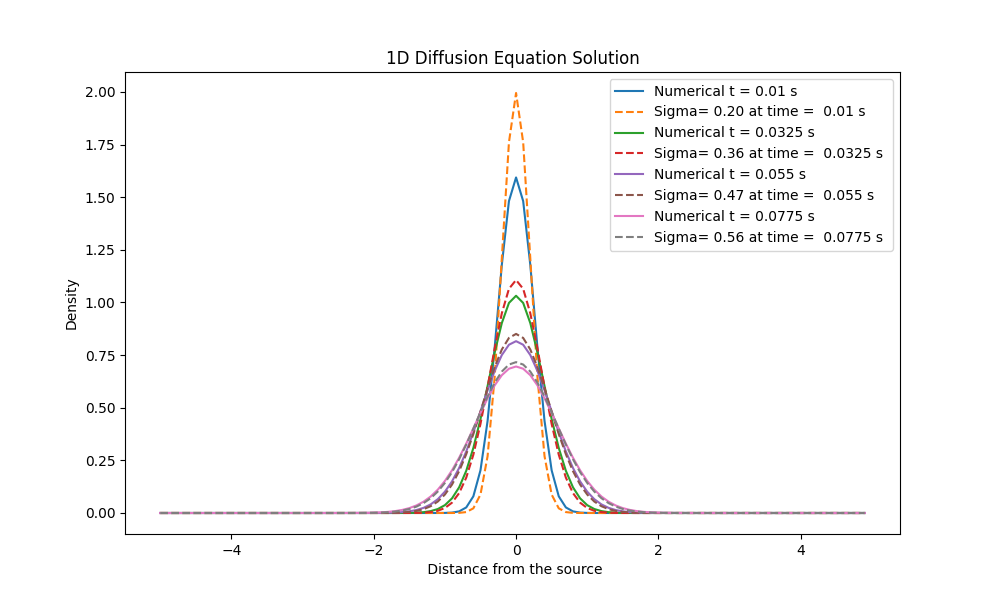
\includegraphics[width=1\textwidth, keepaspectratio]{1D Diffusion Equation Solution.png}
    \caption{1D Diffusion Equation Solution}
    \label{fig:20}
\end{figure}
From Figure~\ref{fig:20}, we can see that the after t = 0.055 seconds the density profile corresponds to a normal distribution.

\section{Mixing of two Gases}
Pseudo-Code:
\begin{enumerate}
    \item \textit{Define a 2D array and give gas A a vlaue of 1 and gas B value of -1 and empty as 0}
    \item \textit{store the indices of gas A,gasB and empty seperatly}
    \item \textit{randomly select gas A or gas B}
    \item \textit{once selected, randomly select the direction in which gas can move, note 4 directions have equal probability}
    \item \textit{check if that space is empty}
    \item \textit{if empty swap the value of 2D array and also the the 2 tuples}
    \item \textit{if not empty, discard and start again}
\end{enumerate}
\subsection{ Set up a 2D grid with 60x40 grid size and run it for longer duration}
\begin{figure}[H]
    \centering
    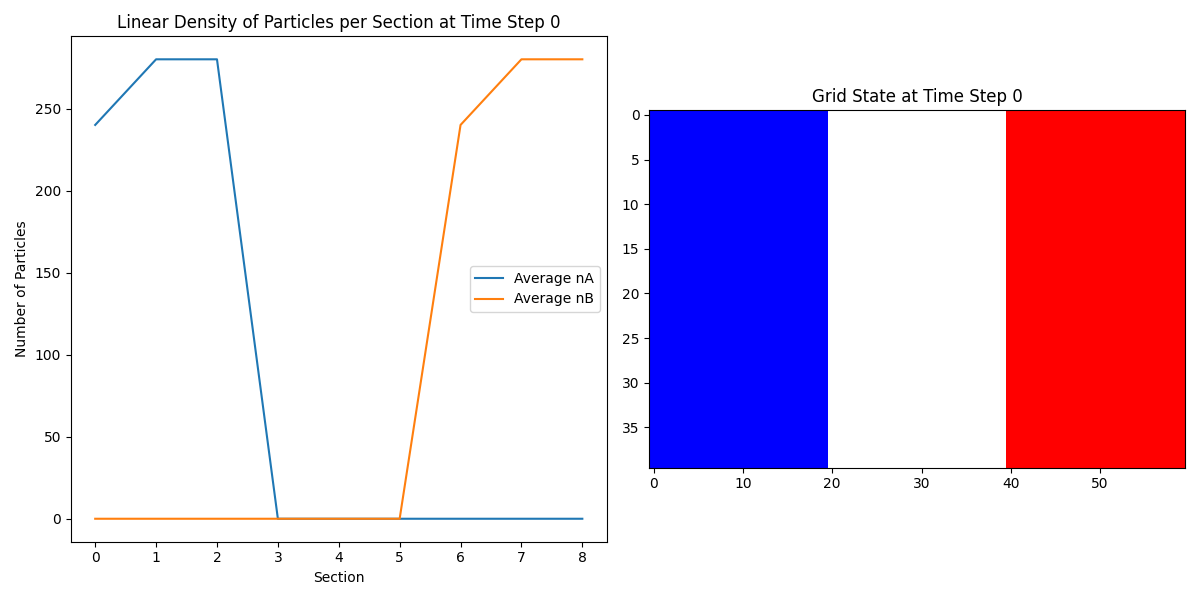
\includegraphics[width=0.75\textwidth, keepaspectratio]{Linear_Density_Grid_After_0_Steps_1_Trial.png}
    \caption{Linear Density and the Grid after 0 Steps}
    \label{fig:21}
\end{figure}
\begin{figure}[H]
    \centering
    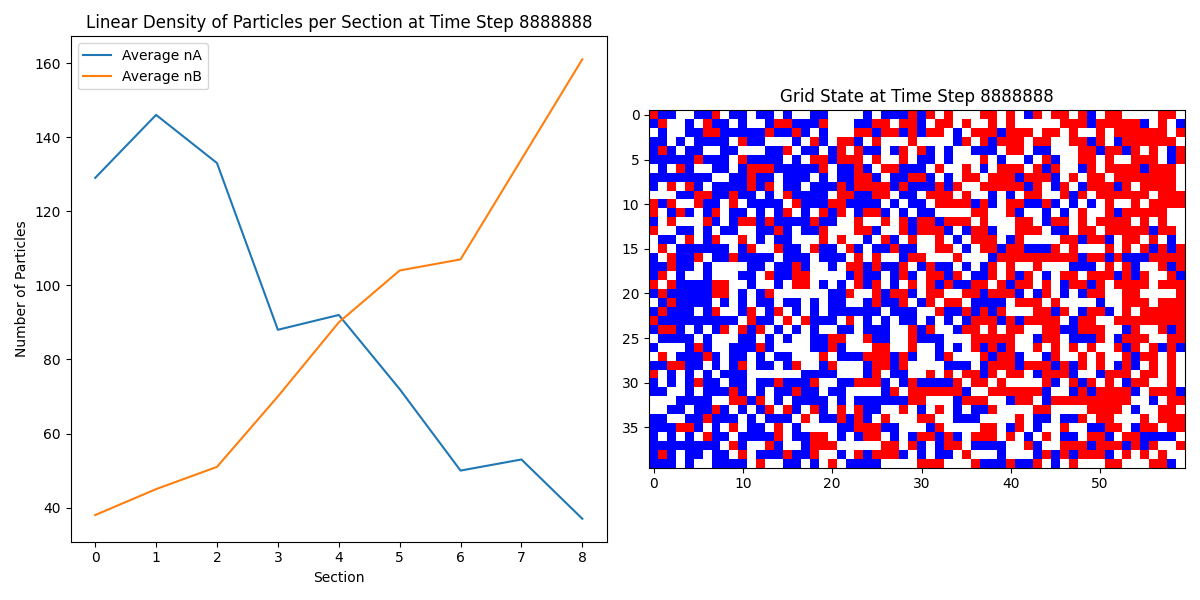
\includegraphics[width=0.75\textwidth, keepaspectratio]{Linear_Density_Grid_After_8888888_Steps_1_Trial.png}
    \caption{Linear Density and the Grid after 8888888 Steps}
    \label{fig:22}
\end{figure}

\subsection{Plot a linear density plot with grid images at some time interval}
\begin{figure}[H]
    \centering
    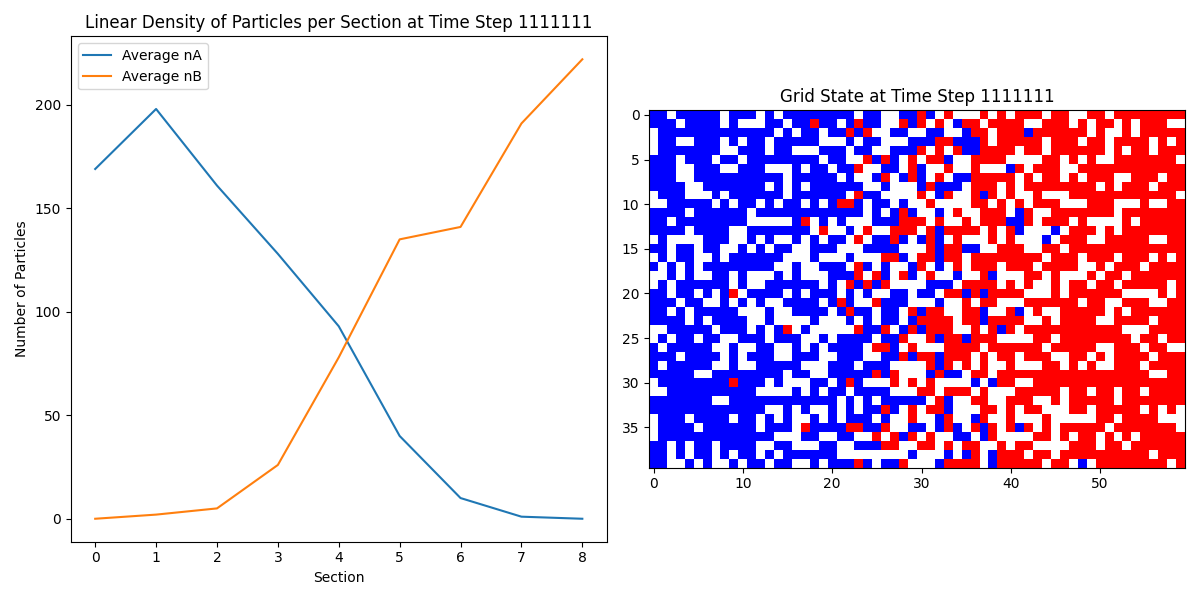
\includegraphics[width=0.75\textwidth, keepaspectratio]{Linear_Density_Grid_After_1111111_Steps_1_Trial.png}
    \caption{Linear Density and the Grid after 1111111 Steps}
    \label{fig:23}
\end{figure}

\begin{figure}[H]
    \centering
    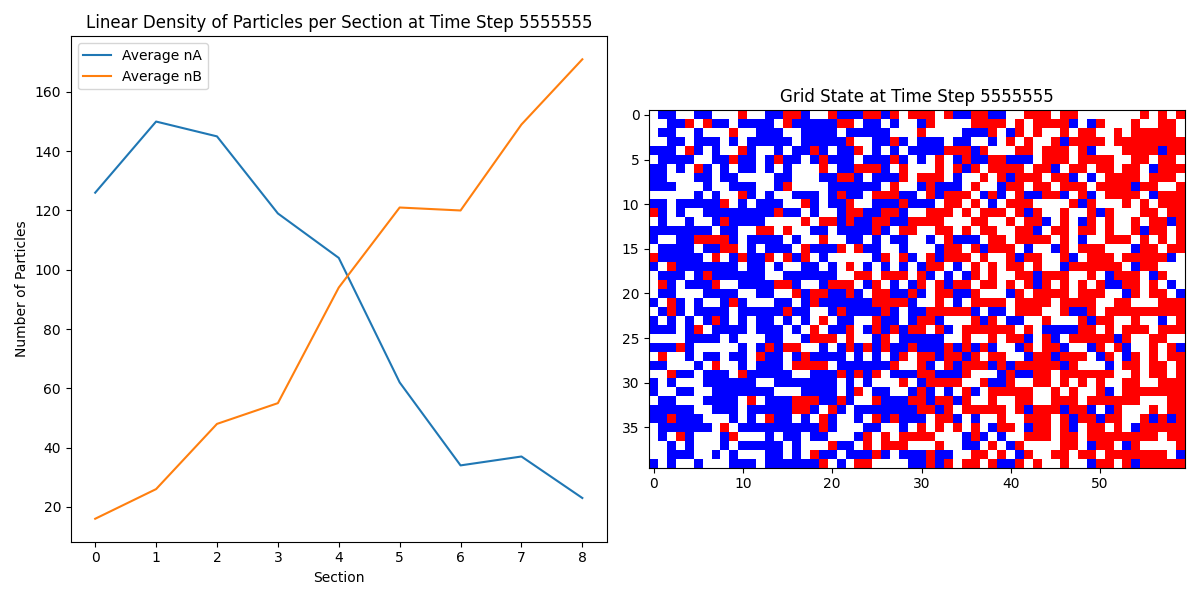
\includegraphics[width=0.75\textwidth, keepaspectratio]{Linear_Density_Grid_After_5555555_Steps_1_Trial.png}
    \caption{Linear Density and the Grid after 5555555 Steps}
    \label{fig:24}
\end{figure}

\begin{figure}[H]
    \centering
    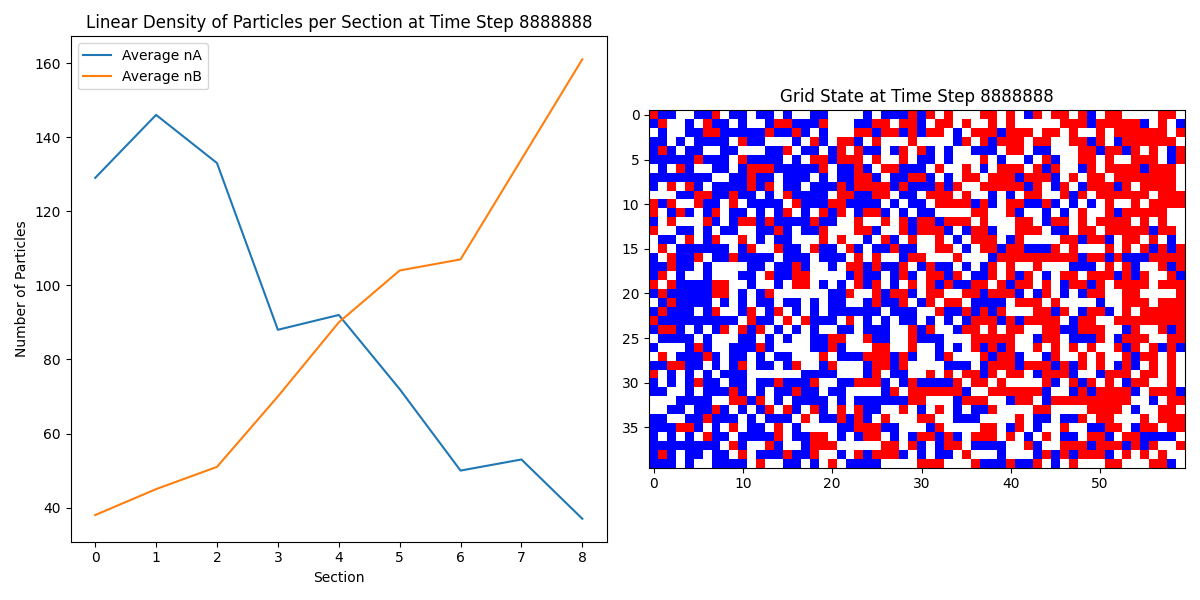
\includegraphics[width=0.75\textwidth, keepaspectratio]{Linear_Density_Grid_After_8888888_Steps_1_Trial.png}
    \caption{Linear Density and the Grid after 8888888 Steps}
    \label{fig:25}
\end{figure}

\begin{figure}[H]
    \centering
    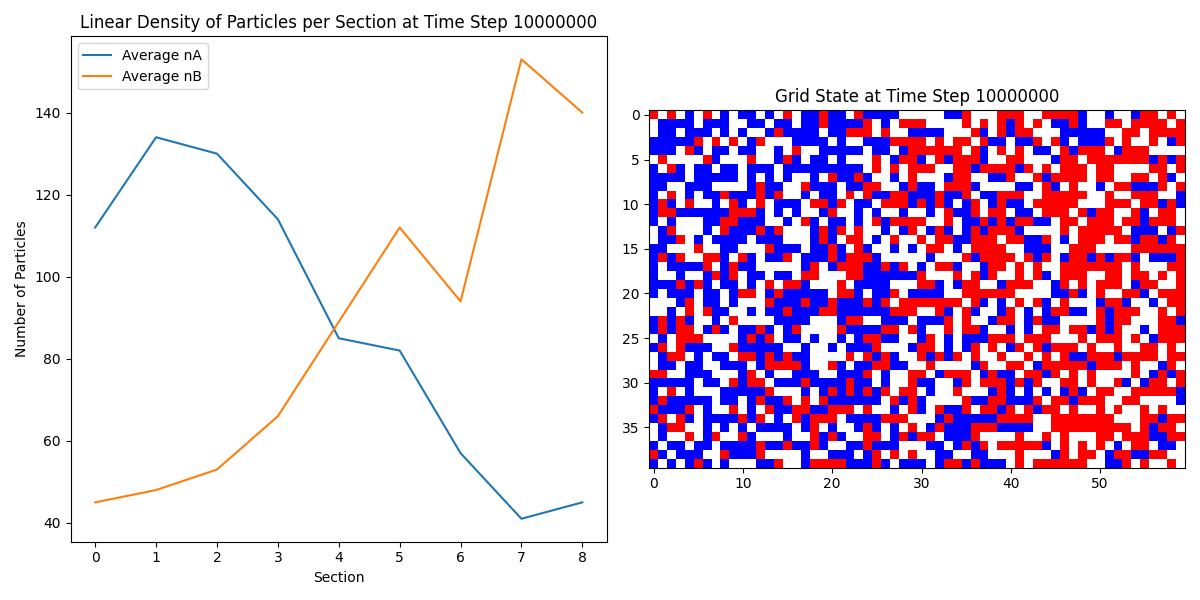
\includegraphics[width=0.75\textwidth, keepaspectratio]{Linear_Density_Grid_After_10000000_Steps_1_Trial.png}
    \caption{Linear Density and the Grid after 10000000 Steps}
    \label{fig:26}
\end{figure}
\subsection{Average the densities over 100 trials for added accuracy and replot the densities}
\begin{figure}[H]
    \centering
    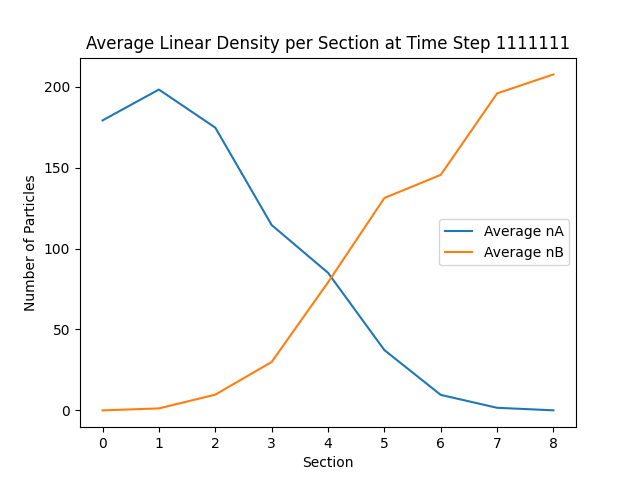
\includegraphics[width=0.5\textwidth, keepaspectratio]{Average_Linear_Density_Grid_After_1111111_Steps_1_Trial.png}
    \caption{Average Linear Density and the Grid after 1111111 Steps}
    \label{fig:27}
\end{figure}

\begin{figure}[H]
    \centering
    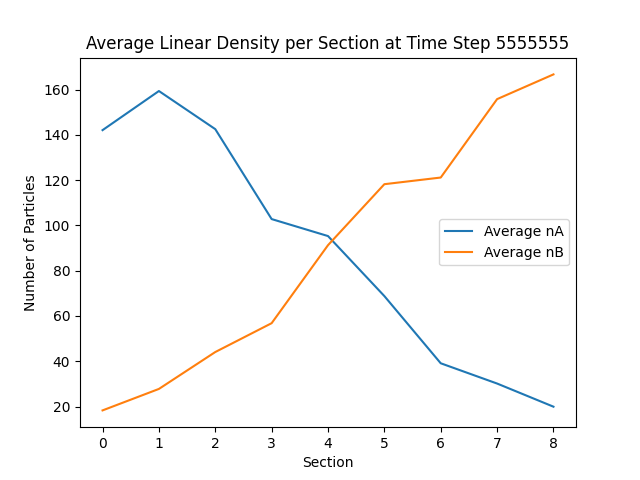
\includegraphics[width=0.5\textwidth, keepaspectratio]{Average_Linear_Density_Grid_After_5555555_Steps_1_Trial.png}
    \caption{Average Linear Density and the Grid after 5555555 Steps}
    \label{fig:28}
\end{figure}

\begin{figure}[H]
    \centering
    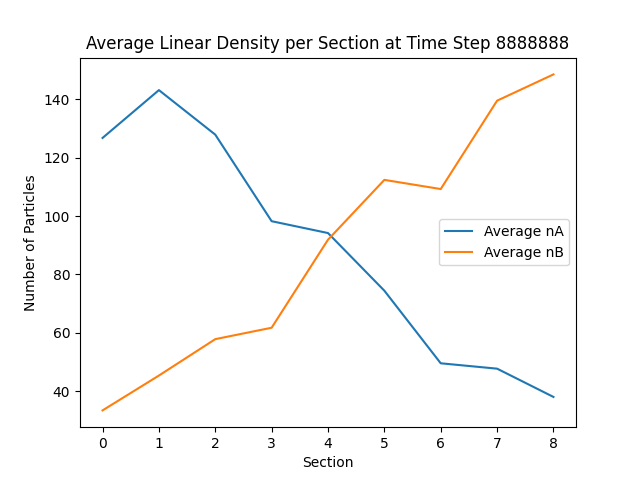
\includegraphics[width=0.5\textwidth, keepaspectratio]{Average_Linear_Density_Grid_After_8888888_Steps_1_Trial.png}
    \caption{Average Linear Density and the Grid after 8888888 Steps}
    \label{fig:29}
\end{figure}

\section{Conclusion}
\begin{enumerate}
    \item From Figure~\ref{fig:10} and Figure~\ref{fig:14} we observed that for getting a smooth Gaussian distribution the number of elements needs to be on higher side.
    \item Figure~\ref{fig:21} and Figure~\ref{fig:22}, we can say the the simulation of gasses mixing is a memory intensive job and we observed almost homogeneous mixture around the end of 10$^7$ iterations
\end{enumerate}

\section*{Contribution}
\begin{enumerate}
    \item Thanks to Alison for helping me with the diffusion problem, specifically for making me understand finite difference algorithm and also for initially i took x$^2$ same as r$^2$, alison pointed out the mistake. And for cross checking out plots
    \item Thanks to Sravya for helping me find the problem in my random walk algorithm. And for cross checking out plots
\end{enumerate}

\begin{thebibliography}{}
\bibitem{ref1} Gaussian Random Number Generator. Available at: \url{https://www.tspi.at/2021/08/17/gaussianrng.html}
\end{thebibliography}

\end{document}